\chapter{Modeling}
\label{ch:modeling}
\begin{figure}[htbp]
\centering
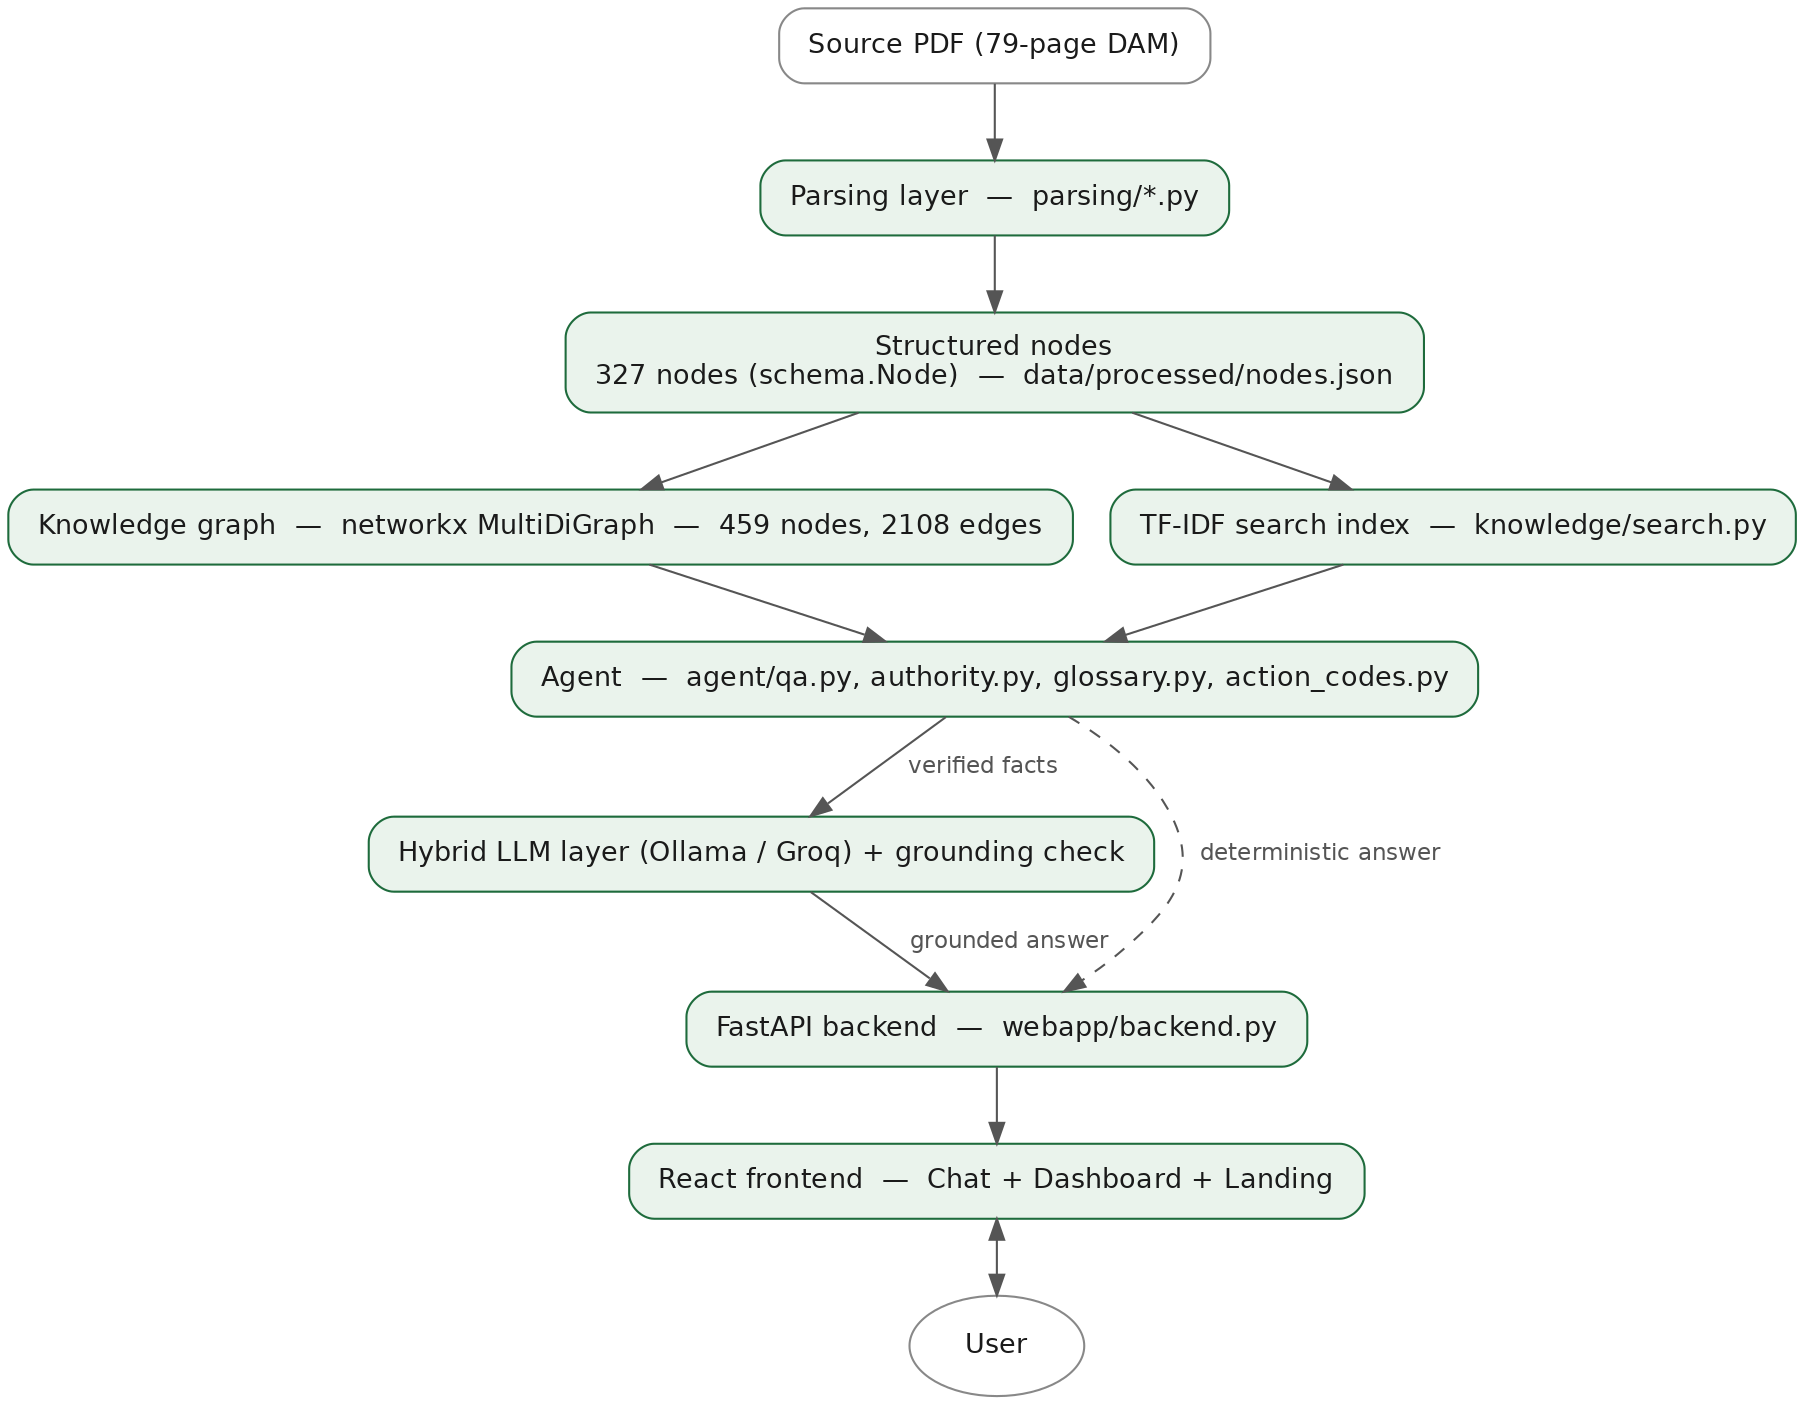
\includegraphics[width=0.82\textwidth,height=0.8\textheight,keepaspectratio]{figures/fig1_architecture.png}
\caption{End-to-end system architecture: source document to user-facing answer.}
\label{fig:fig1_architecture}
\end{figure}
\section{Knowledge graph}
The structured node set is loaded into a \texttt{networkx} \texttt{MultiDiGraph} (\texttt{modeling/\allowbreak{}graph.py}) rather than queried as a flat dictionary, because the project's own founding questions ("who approves X", "who is informed about X") are naturally graph queries — "who is connected to X by a particular labeled edge" — and because a role like "Country Manager / DDG" is a real, recurring entity referenced from dozens of different activities and deserves to be one graph node with one identity, not a string repeated independently in 168 different responsibility lists. A \texttt{MultiDiGraph} (allowing parallel edges) was chosen specifically because one role can hold two different responsibilities on the same activity (e.g. it both checks and later approves), which is two parallel edges, not one edge carrying two labels.

Every DAM node keeps its own id; every distinct canonical role string becomes its own node, namespaced (\texttt{role::...}) so it can never collide with a real DAM id; unresolved responsibilities are attached to one shared placeholder node (\texttt{role::\_\allowbreak{}\_\allowbreak{}unresolved\_\allowbreak{}\_\allowbreak{}}) rather than silently dropped, so a query can still surface that something could not be attributed. Three edge types connect the graph: \texttt{contains} (hierarchy), \texttt{references} (cross-activity redirects, wired only when the target id actually exists inside this document's scope — several real redirects point outside the 79-page document and are correctly left unwired rather than pointed at nothing), and \texttt{responsible\_\allowbreak{}for} (role → activity, carrying the authority code, seniority level, and footnote reference as edge attributes).

The current graph has \textbf{459 nodes} (327 DAM nodes plus 131 distinct role nodes, including the unresolved placeholder) and \textbf{2,108 edges}. It was validated not just by edge count but by reproducing a specific real screenshot exactly: querying the graph for activity 3.111's approvers returns precisely "Origination Sector Manager" (footnote 3) and "Supporting Dept. Division Manager" (footnote 4) — the same two names, in the same order, with the same footnote numbers, as the actual printed table.

\begin{figure}[htbp]
\centering
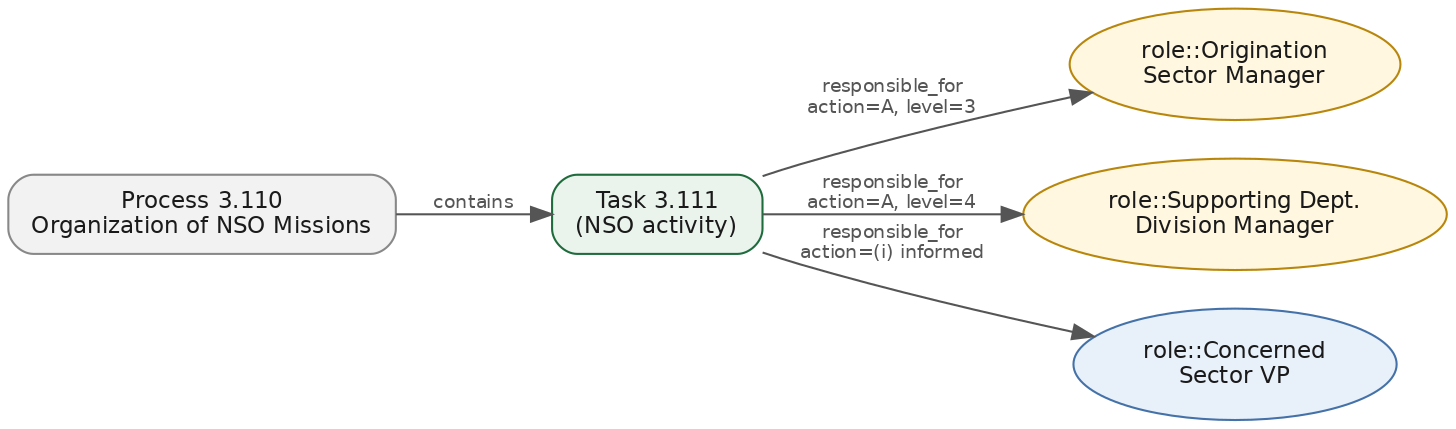
\includegraphics[width=0.82\textwidth,height=0.8\textheight,keepaspectratio]{figures/fig3_graph.png}
\caption{A real excerpt of the knowledge graph around activity 3.111, showing the \texttt{contains} edge from its parent process and the \texttt{responsible\_\allowbreak{}for} edges to its approving and informed roles — the exact structure validated against the real printed table.}
\label{fig:fig3_graph}
\end{figure}
\section{Natural-language understanding}
Two independent resolution paths handle an incoming question (\texttt{knowledge/\allowbreak{}search.py}): an id fast-path that looks for a literal DAM identifier already present in the question text (100\% accurate when it fires, and covers the project's own founding example questions, which are typically phrased with an explicit id), and a TF-IDF lexical fallback for questions phrased by title or description rather than by code.

A separate module, \texttt{agent/\allowbreak{}authority.py}, maps how people actually phrase authority questions ("who signs off on X", "who checks X") onto the DAM's own authority-code structure, reading the code/level definitions directly from the extracted reference data (\texttt{data/\allowbreak{}reference/\allowbreak{}authority\_\allowbreak{}codes.json}) rather than a hand-written vocabulary that could silently drift out of sync with it. The "C" ambiguity found in Data Understanding (Section 6.2) is encoded directly into each intent's matching predicate and covered by a dedicated regression test, so a "consult" question can never be answered with Check/verify facts or vice versa.

On top of this core resolution layer, several real user-experience gaps were found and fixed only through direct testing against real (and sometimes intentionally malformed) questions: plain conversational messages ("hi", "thanks") are recognized and answered directly rather than run through DAM lookup at all; a question containing an id-shaped but non-existent code is explicitly reported as invalid (with real, relevant suggestions) rather than silently falling through to a full-text search that can coincidentally match an unrelated real activity; genuinely vague questions ("mission", "approve") trigger a clarification response listing the top real candidates rather than guessing; and a deliberately conservative deterministic typo-correction layer (\texttt{knowledge/\allowbreak{}typo\_\allowbreak{}correct.py}, threshold-tuned against real observed typos and real observed false positives, e.g. "unrelated" almost incorrectly matching "related") tolerates ordinary misspellings without ever touching the underlying lexical-matching logic itself.

\section{Why TF-IDF over trained embeddings}
With only 327 short titles and no labeled query/title pairs available, training a custom embedding model was ruled out outright: there is nowhere near enough data to beat a general-purpose pretrained embedding model, and doing so anyway would risk visible overfitting rather than a real capability gain — "there was not enough data to justify it" is judged the more defensible answer to give a reviewer than attempting it regardless. Installing a pretrained sentence-embedding library (\texttt{sentence-transformers}, which requires PyTorch) was attempted as the alternative and failed to complete twice in the development sandbox due to the size of the dependency — a real, if environment-specific, signal about deployment weight. TF-IDF via scikit-learn was chosen for reliability and portability (installs in roughly 17 seconds, no heavy dependency, runs anywhere).

This choice is explicitly disclosed as lexical (shared-word) rather than semantic (shared-meaning) matching throughout the system: every resolved answer carries a \texttt{method} field (\texttt{"id"} or \texttt{"text\_\allowbreak{}search"}) so this distinction is visible to any caller, rather than the system silently implying an understanding of meaning it does not have. The consequence — a question phrased with different words than the actual title (e.g. "sign off on" versus "Signature of") scores lower than an exact phrase match — is documented as a known, accepted limitation of this design choice, not treated as a bug to be patched away.

\section{Grounded generation: how the LLM is allowed to touch the answer}
This is the architectural decision most directly traceable back to the Business Understanding success criteria (Section 4.3), and the one most worth explaining carefully, because "integrate an LLM" or "add RAG" can mean two very different things. One option — the textbook interpretation of retrieval-augmented generation — would chunk the source document, embed it, and let an LLM freely reason over whatever text gets retrieved. This was explicitly rejected: it would have quietly undone the entire reason the project exists, since the whole point of building a structured knowledge graph in the first place was to avoid an LLM hallucinating who approves a financial transaction by grounding every answer in a verified data structure instead of raw document search.

The chosen design keeps retrieval exactly as validated in Sections 8.1–8.2 (deterministic, checked against real screenshots) and restricts the LLM to a strictly narrower job: rephrasing facts that retrieval has already found, never deciding what those facts are. \texttt{agent/\allowbreak{}generate.py} builds a system prompt instructing the model to use only the facts supplied and to say so plainly if the fact list is empty, then checks its output against those same facts with a grounding function (\texttt{\_\allowbreak{}mentions\_\allowbreak{}expected\_\allowbreak{}facts}) that requires every role name to survive, verbatim (normalized only for whitespace and case, never abbreviated or paraphrased), in the model's rephrasing. If any name is dropped or altered, the system discards the LLM's answer entirely and falls back to the original deterministic template answer — never a partially-trusted hybrid. Two cases never reach the LLM at all: no provider configured, and no real activity resolved (nothing to phrase, which would only invite the model to invent something plausible-sounding).

This is still legitimately retrieval-augmented generation — the retrieval step existed, was validated, and remains completely unaffected by the LLM's presence; only the generation half of RAG changed.

\begin{figure}[htbp]
\centering
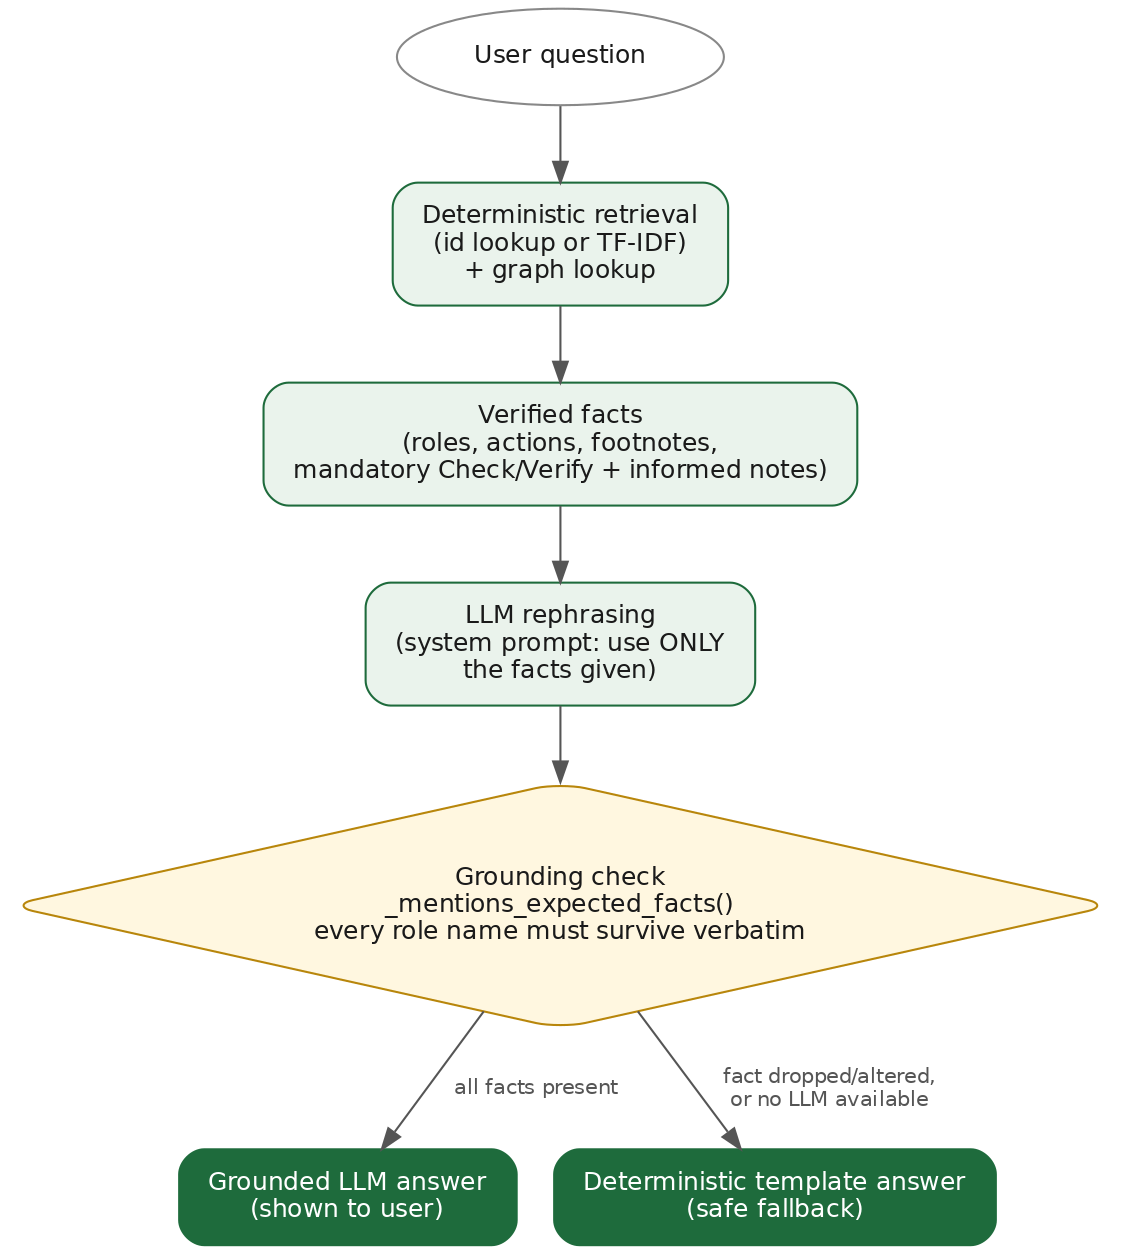
\includegraphics[width=0.82\textwidth,height=0.8\textheight,keepaspectratio]{figures/fig4_grounding.png}
\caption{The grounded-generation flow: an LLM may only rephrase already-verified facts, and any answer that drops or alters a fact is discarded in favor of the safe deterministic template.}
\label{fig:fig4_grounding}
\end{figure}
\section{Hybrid local/cloud LLM layer}
A common interface (\texttt{llm/\allowbreak{}base.py}, one \texttt{chat()} method and one shared failure exception) sits in front of two interchangeable providers: a local Ollama server (default model \texttt{llama3.1}, no network dependency, no cost) and Groq's cloud API (originally \texttt{llama-3.3-70b-versatile}, migrated in September 2026 to \texttt{openai/\allowbreak{}gpt-oss-120b} after the original model was moved to enterprise-only pricing — see Section 10.5). A router resolves a requested mode ("off"/"ollama"/"groq"/"auto") to a concrete provider; "auto" mode was initially set to prefer the free local option and fall back to the cloud API only if the local server was unreachable, then later reversed at the intern's request to prefer the cloud API first (faster, no local setup required for a demo audience) with local as the fallback if the API key is unavailable — a real example of a design choice being revisited once actual usage patterns (a live demo, not a development machine) made the original assumption wrong.

\section{Recent modeling extensions: multi-language, mandatory notes, tone}
Three further modeling-layer capabilities were added in direct response to explicit requests after the initial system was demonstrated (see Section 10.6 for full detail on each, since they were shipped as part of deployment-stage iteration): translating questions and answers across five languages while keeping the underlying English retrieval and grounding check completely unchanged; treating a DAM row's mandatory Check/Verify authority as a fact the agent must always surface even when not directly asked, rather than optional supplementary detail, following an explicit domain-knowledge correction from the intern; and a cheap, pre-filtered LLM classification step that detects a frustrated or confused user and prepends a short, deterministic, language-matched empathetic opener to any response type — never a second free-form generation, so the added warmth carries none of the factual risk the core grounding check exists to prevent.

